%!TeX program = xelatex
\documentclass[UTF8,a4paper,12pt,fontset=windows]{ctexart}

\usepackage[margin=2.45cm,headheight=15pt]{geometry}
\usepackage{graphicx}
\usepackage{booktabs}
\usepackage{array}
\usepackage{amsmath}
\usepackage{float}
\usepackage{subcaption}
\usepackage{tikz}
\usetikzlibrary{arrows.meta,positioning,shapes.geometric}
\usepackage{xcolor}
\usepackage{fancyhdr}
\usepackage{hyperref}

\definecolor{reportblue}{RGB}{23,63,105}
\definecolor{reportlight}{RGB}{236,243,249}
\hypersetup{hidelinks,pdftitle={图像预处理与人脸分割定位实验报告},pdfauthor={浙江大学数字信号处理综合实验}}
\setlength{\parindent}{2em}
\setlength{\parskip}{0.28em}
\renewcommand{\arraystretch}{1.25}
\captionsetup{font=small,labelfont=bf}
\pagestyle{fancy}
\fancyhf{}
\fancyhead[L]{数字信号处理综合实验}
\fancyhead[R]{图像预处理与人脸分割定位}
\fancyfoot[C]{\thepage}
\renewcommand{\headrulewidth}{0.4pt}

\begin{document}
\begin{titlepage}
  \thispagestyle{empty}
  \centering
  \vspace*{1.35cm}
  
\includegraphics[width=0.16\textwidth]{figures/zju_logo.png}\par
  \vspace{0.55cm}
  
\includegraphics[width=0.40\textwidth]{figures/zju_char.png}\par
  \vspace{1.45cm}
  {\zihao{1}\bfseries 数字信号处理综合实验\par}
  \vspace{0.55cm}
  {\zihao{2}\bfseries 图像预处理与人脸分割定位\par}
  \vspace{0.28cm}
  {\zihao{3}实验报告\par}
  \vspace{1.45cm}
  \rule{0.76\textwidth}{0.7pt}\par
  \vspace{0.8cm}
  \begin{tabular}{>{\raggedleft\arraybackslash}p{3.6cm}p{7.0cm}}
    姓\qquad 名： & \hrulefill\\[0.48cm]
    学\qquad 号： & \hrulefill\\[0.48cm]
    学\qquad 院： & \hrulefill\\[0.48cm]
    指导教师： & \hrulefill\\
  \end{tabular}
  \vfill
  {\large 2026 年 10 月\par}
\end{titlepage}

\pagenumbering{Roman}
\tableofcontents
\clearpage
\pagenumbering{arabic}

\section{实验目标与系统接口}
\subsection{任务范围}
课程防疲劳瞌睡系统以摄像头视频流为输入，后续还包含眼部检测、跟踪和疲劳判定。本实验只实现其中两个连续插件：\texttt{ImagePrepare} 负责共享缓冲区初始化与图像降采样，\texttt{FaceLocator} 负责肤色分割、人脸区域定位及颈部等非面部区域的排除。实验不实现眨眼检测、眼鼻跟踪或报警，因此本文的结果也不代表完整防瞌睡系统的检测效果。

原课程工程提供插件框架，但初始版本的 \texttt{ImagePrepare::ON\_PLUGINRUN} 尚未完成实际的缓冲区和图像处理；本实验补全了这部分逻辑，并实现了人脸分割定位。两个插件继续使用课程规定的逐帧入口和共享缓冲区，不改变主程序与插件之间的函数接口。

\subsection{数据流与坐标系}
主程序向插件传入 \(W\times H\) 的 YUV422 planar 图像：Y 平面大小为 \(WH\)，U、V 平面各为 \(WH/2\)。在实验使用的 \(640\times480\) 帧上，\texttt{ImagePrepare} 生成 \(320\times120\) 的降采样彩色图；其色度平面及人脸二值 mask 均为 \(160\times120\)。\texttt{FaceLocator} 使用色度平面做肤色判断，并把结果换算回课程要求的降采样彩色图坐标系。

\begin{figure}[H]
  \centering
  \begin{tikzpicture}[node distance=8mm and 9mm,>=Latex,
    box/.style={draw=reportblue,rounded corners=3pt,fill=reportlight,align=center,
                minimum height=1.1cm,text width=2.9cm,font=\small}]
    \node[box] (input) {摄像头与主程序\\YUV422 planar};
    \node[box,right=of input] (prepare) {\texttt{ImagePrepare}\\缓冲区与降采样};
    \node[box,right=of prepare] (segment) {\texttt{FaceLocator}\\肤色分割与连通域};
    \node[box,below=of segment] (oval) {面部关键点\\轮廓约束精修};
    \node[box,left=of oval] (output) {面部 mask、包围框\\肤色像素数};
    \draw[->,thick] (input) -- (prepare);
    \draw[->,thick] (prepare) -- (segment);
    \draw[->,thick] (segment) -- (oval);
    \draw[->,thick] (oval) -- (output);
  \end{tikzpicture}
  \caption{本实验实现的数据处理流程}
  \label{fig:flow}
\end{figure}

\section{图像预处理插件 \texttt{ImagePrepare}}
\subsection{共享缓冲区初始化}
主程序提供长度为 \(4WH\) 字节的共享缓冲区。插件先检查输入指针、尺寸约束和固定区容量，再在缓冲区内依次安排 \texttt{BUF\_STRUCT}、原图彩色副本、原图灰度副本、降采样彩色图、降采样灰度图、临时二值 mask、\texttt{OTHER\_VARS} 和余下的临时空间。仅在首次运行或尺寸改变时重新初始化结构体和指针；逐帧更新显示指针与图像内容。这样，下游插件读取的是同一套稳定的缓存位置。

\begin{table}[H]
  \centering
  \caption{共享缓冲区中的主要图像数据}
  \label{tab:buffers}
  \begin{tabular}{p{3.2cm}p{3.2cm}p{6.1cm}}
    \toprule
    数据 & 尺寸或容量 & 用途\\
    \midrule
    原图彩色副本 & \(2WH\) 字节 & 连续保存 Y、U、V 原始平面\\
    原图灰度副本 & \(WH\) 字节 & 保存完整分辨率的 Y 平面\\
    降采样彩色图 & \(WH/4\) 字节 & Y 为 \((W/2)\times(H/4)\)，U/V 各为 \((W/4)\times(H/4)\)\\
    降采样灰度图 & \(WH/16\) 字节 & 保存 \((W/4)\times(H/4)\) 的 Y 采样\\
    临时二值 mask & \(WH/16\) 字节 & 保存与降采样色度同尺寸的分割结果\\
    \bottomrule
  \end{tabular}
\end{table}

\subsection{降采样与坐标关系}
降采样彩色图的亮度值直接取自原图 \(Y(2x,4y)\)。输入 U、V 平面的宽度为 \(W/2\)，输出色度像素分别取输入色度平面坐标 \((2x,4y)\)。另外，\(W/4\times H/4\) 的灰度图取 \(Y(4x,4y)\)。这里使用直接抽样，没有另加插值或滤波，因而坐标关系可逐像素复核。

\begin{figure}[H]
  \centering
  \begin{tikzpicture}[>=Latex,font=\small,
    plane/.style={draw=reportblue,fill=reportlight,rounded corners=2pt,
                  align=center,minimum width=3.6cm,minimum height=1.25cm}]
    \node[plane] (srcy) at (0,2.0) {原始 Y\\\(W\times H\)};
    \node[plane] (srcuv) at (0,0) {原始 U、V\\各 \((W/2)\times H\)};
    \node[plane] (srcgray) at (0,-2.0) {原始 Y\\\(W\times H\)};
    \node[plane] (dsty) at (7,2.0) {降采样 Y\\\((W/2)\times(H/4)\)};
    \node[plane] (dstuv) at (7,0) {降采样 U、V\\各 \((W/4)\times(H/4)\)};
    \node[plane] (gray) at (7,-2.0) {灰度图\\\((W/4)\times(H/4)\)};
    \draw[->,thick] (srcy.east) -- node[above]{\(Y(2x,4y)\)} (dsty.west);
    \draw[->,thick] (srcuv.east) -- node[above]{色度坐标 \((2x,4y)\)} (dstuv.west);
    \draw[->,thick] (srcgray.east) -- node[above]{\(Y(4x,4y)\)} (gray.west);
  \end{tikzpicture}
  \caption{亮度与色度平面的降采样关系}
  \label{fig:sampling}
\end{figure}

\subsection{接口验证}
使用 \(640\times480\) 的合成 YUV 帧直接调用编译后的插件，逐像素核查降采样 Y/U/V 坐标、原始平面副本、缓冲区边界和输入不变性，契约测试输出为 \texttt{ImagePrepare buffer and sampling contract: PASS}。摄像头测试中，主程序经格式协商获得 \(640\times480\) 帧；仅启用预处理插件时，窗口右上角显示 \(320\times120\) 的降采样彩色图。这两项检查分别验证了数组关系和实际采集链路。

\section{人脸分割定位插件 \texttt{FaceLocator}}
\subsection{肤色形态学与最大连通域分割}
基础方法在降采样 U、V 平面上逐像素应用讲义给出的经验阈值：
\begin{equation}
  M_0(x,y)=
  \begin{cases}
    255,&85\leq U(x,y)\leq126\ \text{且}\ 130\leq V(x,y)\leq165,\\
    0,&\text{其他情况}.
  \end{cases}
\end{equation}
随后依次执行 \(3\times3\) 矩形结构元素开运算和 \(7\times7\) 矩形结构元素闭运算，以去除孤立噪点并填补局部空洞。实现将方形腐蚀、膨胀拆为水平和垂直扫描；在结果不变的前提下减少重复邻域访问。对处理后的二值图进行四邻域连通域标记，保留像素数最多的区域，计算其包围框及像素数。

输出的 \texttt{rcnFace} 属于 \(320\times120\) 降采样彩色图坐标系：mask 横坐标与宽度乘以 2，纵坐标与高度保持不变；\texttt{nFacePixelNum} 同样按课程接口约定将 mask 像素数乘以 2。显示框再换算到原始视频坐标。插件把二值结果扩展写入降采样图的 Y 平面，保持 U/V 平面不变，便于后续模块继续使用色度信息。

基础方法可找到主要肤色区域，但面部与颈部常在肤色 mask 中连通，最大连通域无法单凭连通性确定下巴边界。图\ref{fig:first-frame}的基础包围框下缘进入颈部，说明还需对面部范围施加更明确的约束。

\subsection{面部关键点轮廓约束分割}
精修方法使用 MediaPipe Face Landmarker 检测面部关键点。该组件采用机器学习模型，可从图像获得面部关键点\cite{mediapipe-guide}；本实验用关键点构成面部外轮廓\cite{mediapipe-connections}。插件从原始 YUV 帧转换出 \(320\times240\) 的 RGB 图，经常驻 Python 进程获得下巴点和轮廓点，再把它们映射到 \(160\times120\) 的 mask 坐标。

设 \(M_{\mathrm{skin}}\) 为肤色分割及头部区域精修后的 mask，\(P_{\mathrm{face}}\) 为关键点围成的面部多边形，则最终 mask 为
\begin{equation}
  M_{\mathrm{face}}(x,y)=M_{\mathrm{skin}}(x,y)\land
  \mathbf{1}\bigl[(x,y)\in P_{\mathrm{face}}\bigr].
\end{equation}
这样保留轮廓内的肤色像素，排除轮廓外与脸相连的颈部及背景肤色。随后重新统计非零像素和包围框。采用交集而非直接填满轮廓，也避免把眼镜、头发等非肤色位置一律计入肤色 mask。

下巴关键点必须落在现有肤色框内，且交集不能异常缩小；否则不应用轮廓结果。模型缺失、检测失败、响应超时或轮廓检查未通过时，插件沿用现有的几何区域精修结果，并继续输出课程接口字段。该回退保证插件在附加模型不可用时仍能给出传统方法的结果，但回退结果不能视为完成了同等精度的颈部分离。

\section{实验结果与分析}
\subsection{预处理与样本选择}
测试视频长度约 22.34 秒，原分辨率为 \(1280\times720\)。离线脚本按每秒 2 帧抽样，将画面缩放为 \(640\times360\) 并在上下补边到 \(640\times480\)，共得到 45 帧。其中第 023、036 帧的基础检测框只覆盖红色背景，被排除出下颌轮廓对照；其余 43 帧均进入对照。该选择规则说明后续数字仅描述已入选画面，不能代替全视频检出率。

\subsection{基础分割与面部轮廓对照}
图\ref{fig:first-frame}同时给出同一帧的原图、基础包围框、面部轮廓及两个二值 mask。基础框包含下巴以下区域，面部轮廓的下缘接近真实下巴。最终 mask 仍保留轮廓内的肤色，却减少了颈部像素。

\begin{figure}[H]
  \centering
  \begin{subfigure}[t]{0.31\textwidth}\centering
    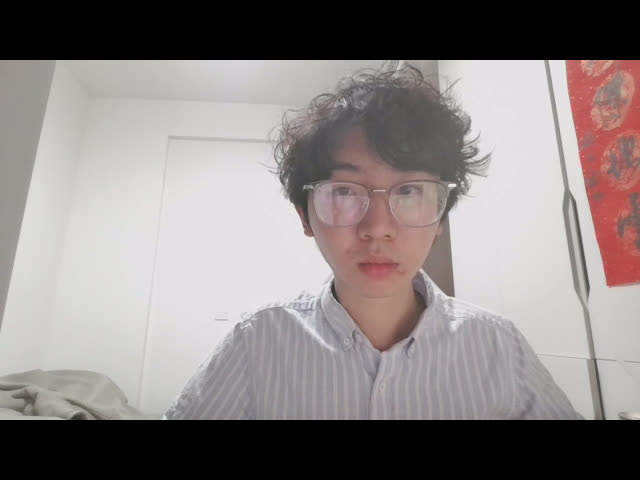
\includegraphics[width=\linewidth]{figures/original_001.jpg}
    \caption{原始画面}
  \end{subfigure}\hfill
  \begin{subfigure}[t]{0.31\textwidth}\centering
    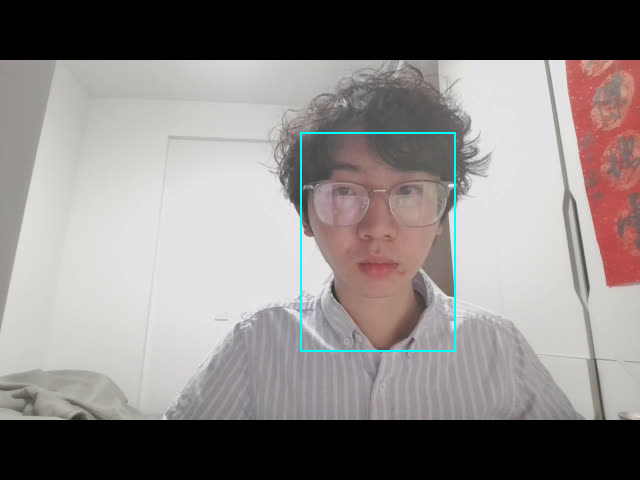
\includegraphics[width=\linewidth]{figures/baseline_box_001.jpg}
    \caption{基础方法包围框}
  \end{subfigure}\hfill
  \begin{subfigure}[t]{0.31\textwidth}\centering
    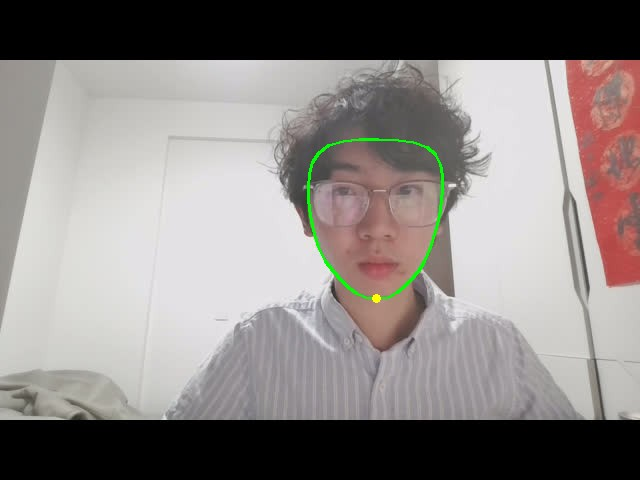
\includegraphics[width=\linewidth]{figures/face_oval_001.jpg}
    \caption{面部轮廓与下巴点}
  \end{subfigure}
  \par\vspace{0.35cm}
  \begin{subfigure}[t]{0.38\textwidth}\centering
    
\includegraphics[width=0.84\linewidth]{figures/baseline_mask_001.png}
    \caption{基础肤色 mask}
  \end{subfigure}\hspace{0.07\textwidth}
  \begin{subfigure}[t]{0.38\textwidth}\centering
    
\includegraphics[width=0.84\linewidth]{figures/face_mask_001.png}
    \caption{轮廓约束后的 mask}
  \end{subfigure}
  \caption{第 001 帧的原图、定位结果与二值分割对照}
  \label{fig:first-frame}
\end{figure}

第 026 帧中人物偏向画面右侧，基础框仍延伸到颈部；第 035 帧的面部与下方肤色连通更明显。图\ref{fig:more-frames}显示，在这两个入选帧上，面部轮廓均使最终 mask 的下缘收回到下颌附近。

\begin{figure}[H]
  \centering
  \begin{subfigure}[t]{0.31\textwidth}\centering
    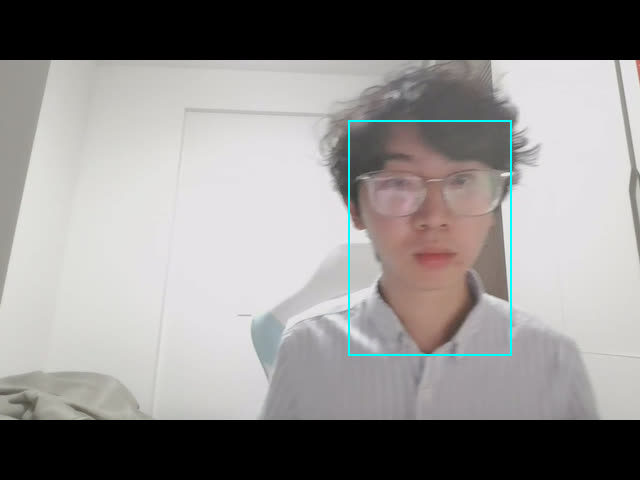
\includegraphics[width=\linewidth]{figures/baseline_box_026.jpg}
    \caption{第 026 帧：基础框}
  \end{subfigure}\hfill
  \begin{subfigure}[t]{0.31\textwidth}\centering
    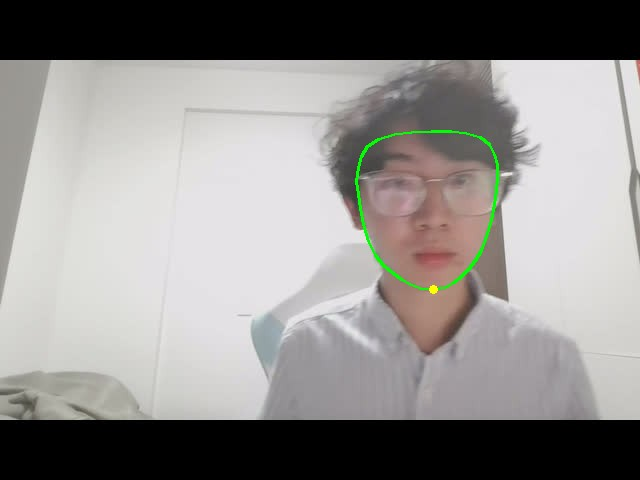
\includegraphics[width=\linewidth]{figures/face_oval_026.jpg}
    \caption{第 026 帧：面部轮廓}
  \end{subfigure}\hfill
  \begin{subfigure}[t]{0.31\textwidth}\centering
    
\includegraphics[width=0.72\linewidth]{figures/face_mask_026.png}
    \caption{第 026 帧：最终 mask}
  \end{subfigure}
  \par\vspace{0.4cm}
  \begin{subfigure}[t]{0.31\textwidth}\centering
    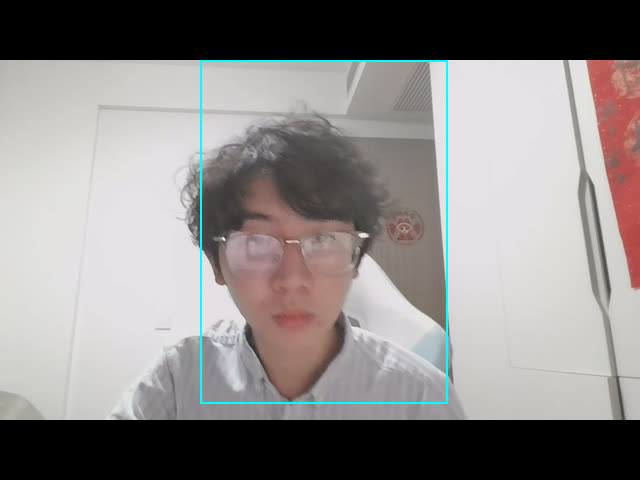
\includegraphics[width=\linewidth]{figures/baseline_box_035.jpg}
    \caption{第 035 帧：基础框}
  \end{subfigure}\hfill
  \begin{subfigure}[t]{0.31\textwidth}\centering
    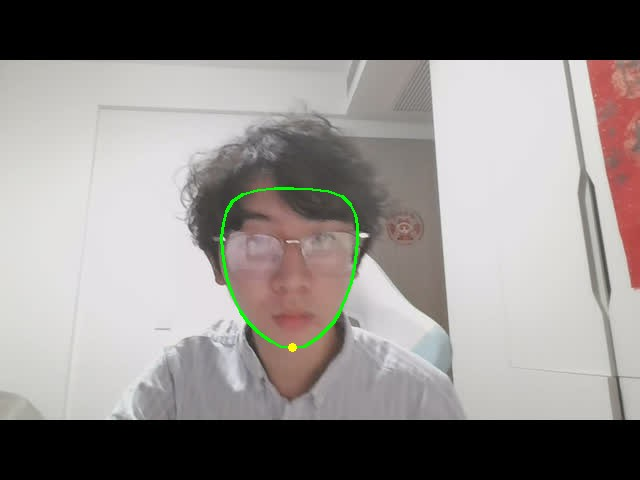
\includegraphics[width=\linewidth]{figures/face_oval_035.jpg}
    \caption{第 035 帧：面部轮廓}
  \end{subfigure}\hfill
  \begin{subfigure}[t]{0.31\textwidth}\centering
    
\includegraphics[width=0.72\linewidth]{figures/face_mask_035.png}
    \caption{第 035 帧：最终 mask}
  \end{subfigure}
  \caption{另两帧的基础框、面部轮廓与最终二值 mask}
  \label{fig:more-frames}
\end{figure}

\subsection{像素统计与适用边界}
表\ref{tab:results}统一按 \(160\times120\) 的二值 mask 像素数计数。课程接口输出的肤色像素数已乘以 2，不能与表中数值直接混用。三个例子的面积均下降；对全部 43 张入选帧，面部关键点均返回有效轮廓，最终 mask 的像素数均低于基础方法。离线关键点检测调用平均耗时约 8.8 ms。

\begin{table}[H]
  \centering
  \caption{代表帧的二值 mask 面积对照}
  \label{tab:results}
  \begin{tabular}{cccc}
    \toprule
    帧号 & 基础肤色区域/像素 & 面部轮廓约束后/像素 & 减少比例\\
    \midrule
    001 & 1366 & 939 & 31.3\%\\
    026 & 1531 & 1013 & 33.8\%\\
    035 & 2649 & 1086 & 59.0\%\\
    \bottomrule
  \end{tabular}
\end{table}

面积减少只证明裁剪发生，不能单独证明每个像素均被正确分类。现有样本来自同一段视频，且两帧基础误检已被排除；尚缺少跨人物、光照、转头和遮挡条件下的人工真值。面部关键点方法还依赖外部模型和本机 Python 环境。以上限制应与局部可视化效果一起理解。

\section{总结}
本实验补全了 \texttt{ImagePrepare} 插件的共享缓冲区初始化与 YUV 降采样，使课程工程能够向后续插件提供可核对坐标的图像数据；在 \texttt{FaceLocator} 中实现肤色阈值、形态学和连通域定位，并加入面部关键点轮廓约束，改善了所选视频中面部与颈部连通造成的分割范围过大问题。

\begin{thebibliography}{9}
  \bibitem{course-material} 浙江大学《数字信号处理综合实验教程（2025 年版）》，实验 5：防疲劳瞌睡系统的设计。
  \bibitem{mediapipe-guide} Google AI Edge, \emph{Face landmark detection guide}.\par
  \url{https://developers.google.com/edge/mediapipe/solutions/vision/face_landmarker}.
  \bibitem{mediapipe-connections} Google AI Edge, \emph{FaceLandmarksConnections API}.\par
  \url{https://ai.google.dev/edge/api/mediapipe/python/mp/tasks/vision/FaceLandmarksConnections}.
\end{thebibliography}

\end{document}
